%!TEX root = ../MasterThesis.tex

\section{Concept of System}
\label{sec:system_concept}

Based on the explanations in Chapter~\ref{cha:context_analysis}, and especially the scope definition for this Master thesis in Section~\ref{sec:scope_thesis}, the collaborative system for investigating E-commerce fraud incidents have to answer the central question:\@

\begin{quotation}
    \textit{Is this really a fraudulent E-commerce transaction?}
\end{quotation}

The relevant stakeholders, that need to be involved in the investigation process, are:\@

\begin{enumerate}
    \item \textbf{merchant}, who can provide additional information of each E-commerce transaction in question
    \item \textbf{\gls{PSP}/issuer}, whose offer information about the credit card usage pattern and the original credit card owner
    \item \textbf{\gls{LSP}}, who can offer information about whether the order has already been shipped or not, and in the former case to whom it has been handed over
    \item \textbf{\gls{ISP}}, who can on request give hints whether a consumer has fallen victim to a phishing attack based on her Internet access logs
\end{enumerate}

Ideally each of them would make parts of their internal data structures available for the other participants to access and query for. This would allow the stakeholder, who has to authorize or validate a suspecious credit card payment, to analyse all available information, as depicted in the Figure~\ref{fig:images_system_overview}.\@

\begin{figure}[H]
	\centering
		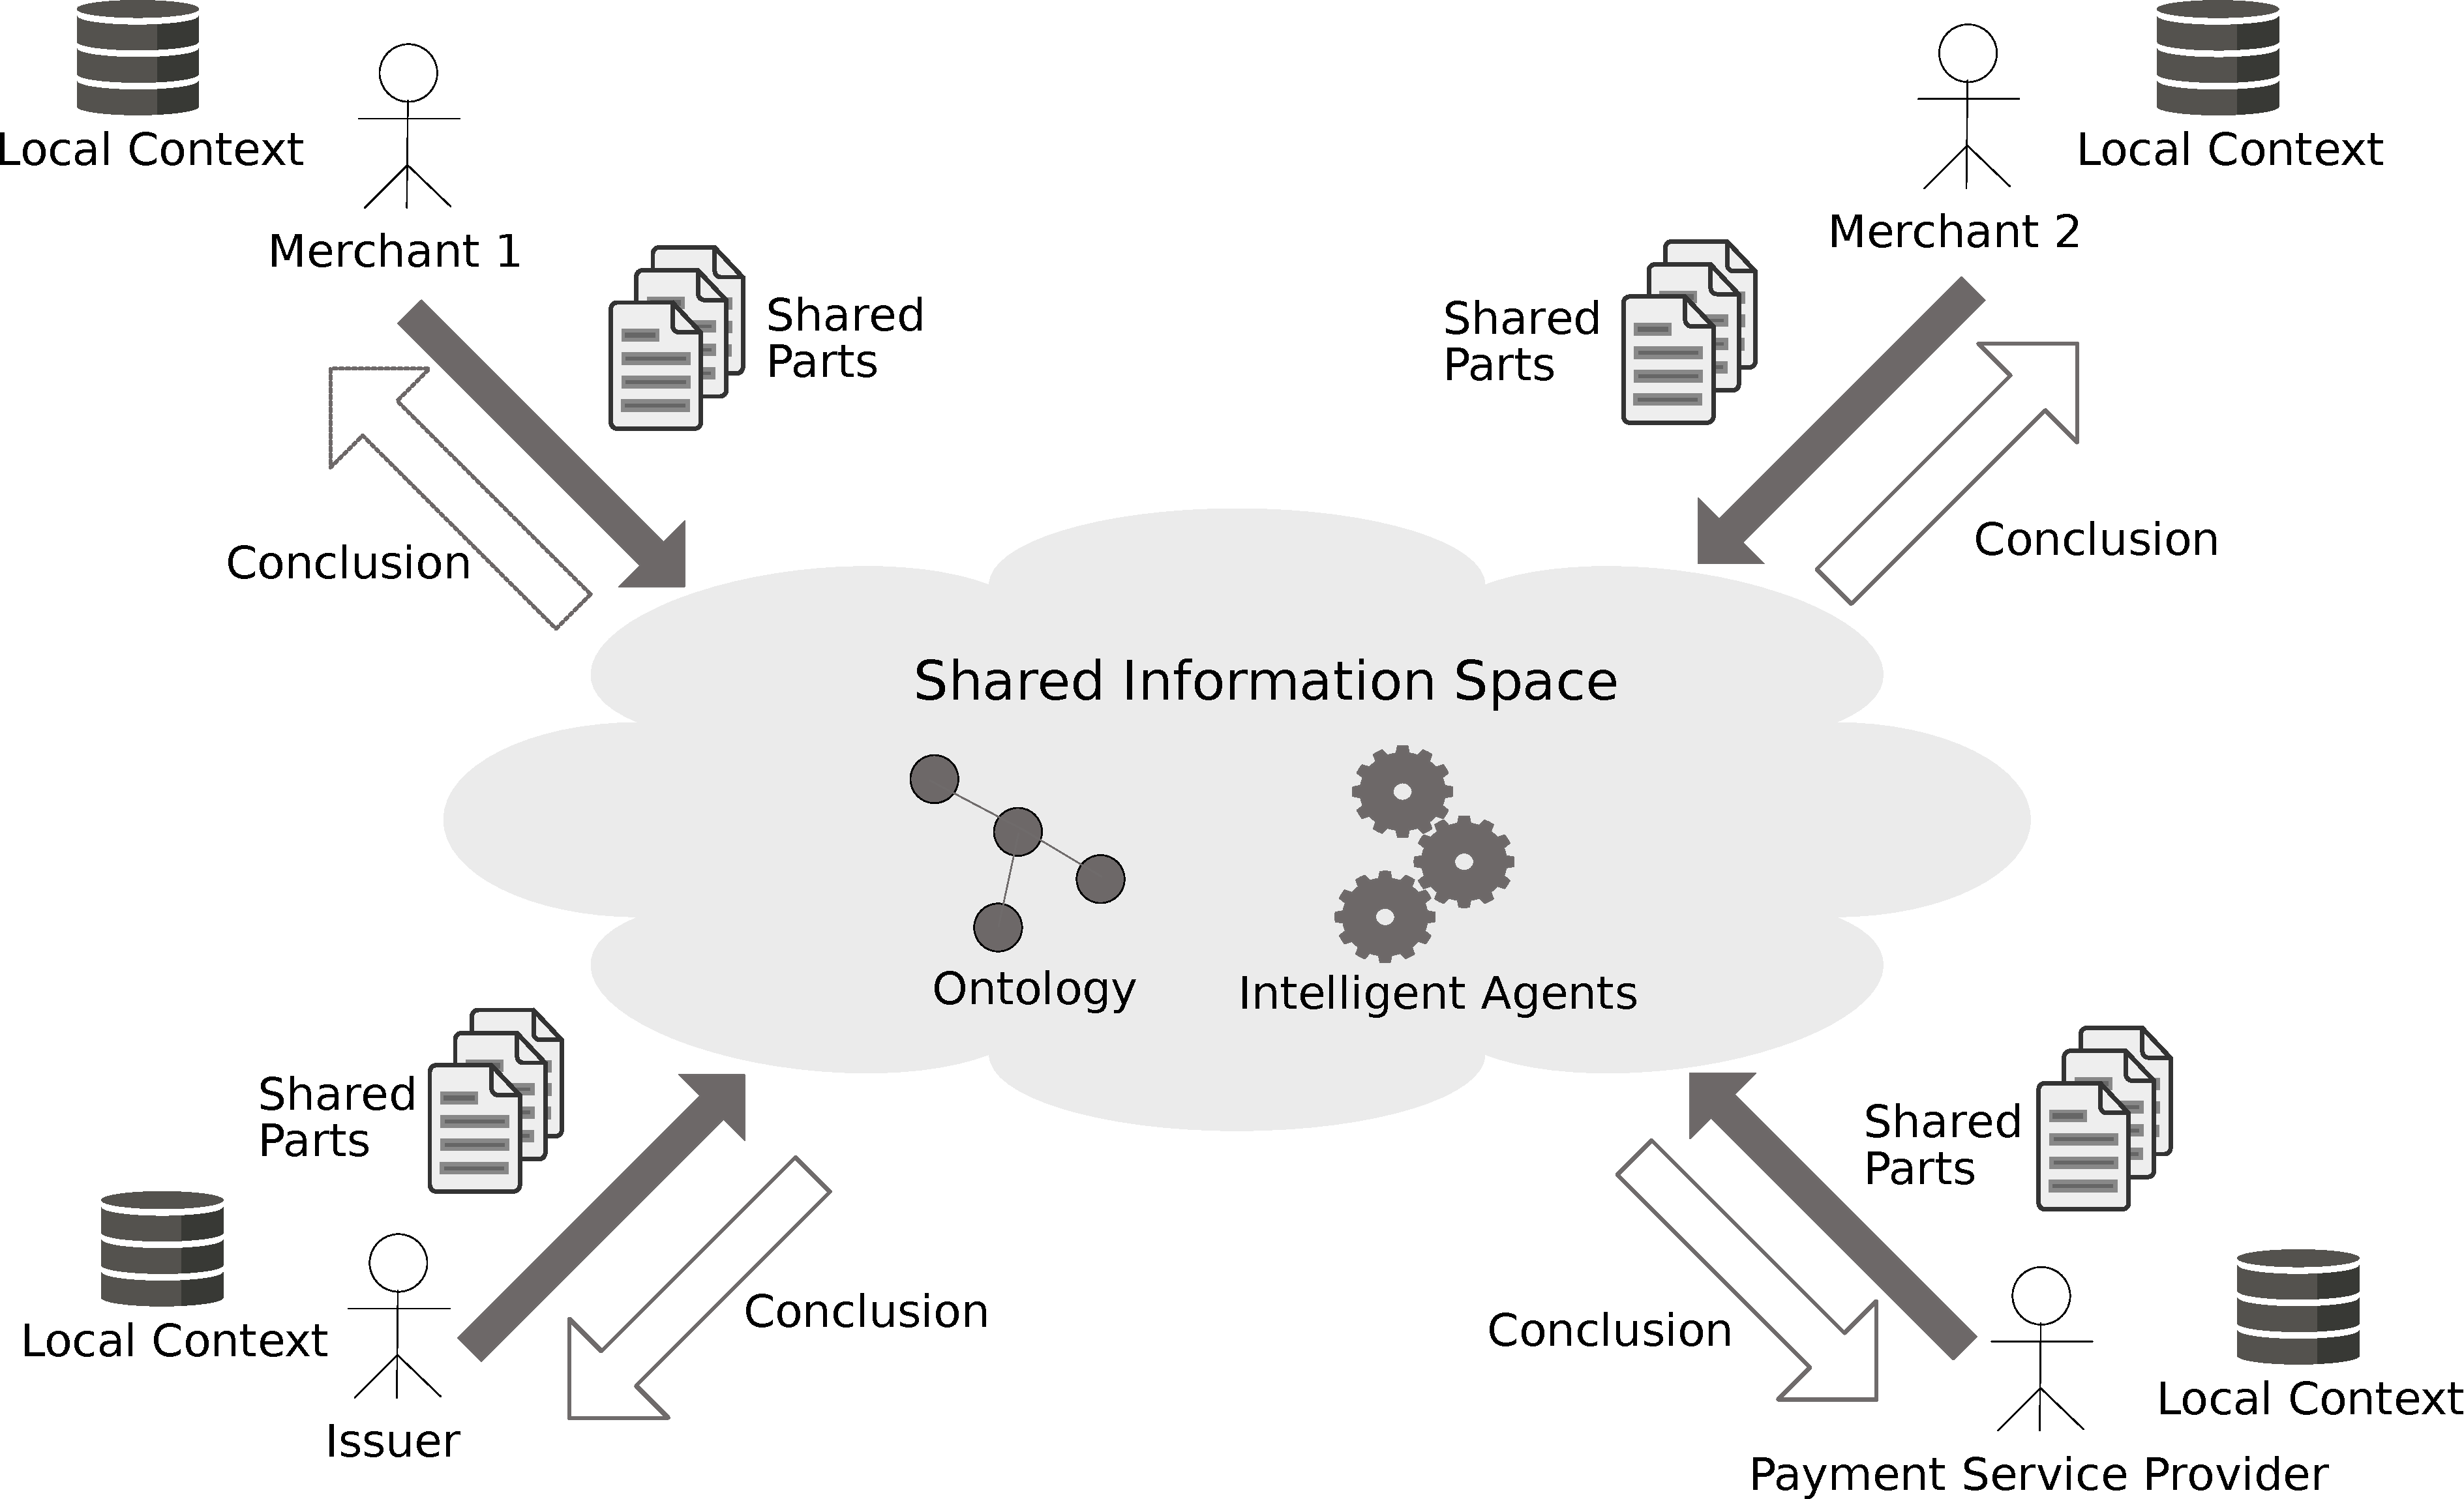
\includegraphics[width=0.9\columnwidth]{images/system_overview.pdf}
	\caption{System Overview}
\label{fig:images_system_overview}
\end{figure}

Due to the fact that data from various sources has to be combined into a shared understanding of the E-commerce activities of a consumer, there is the need to harmonize and transform the information into a shared data model. Based on the discussions in Chapter~\ref{cha:context_analysis} and the analysis of the information each stakeholder holds and transmits to others, the following initial information schema can be conducted (see Figure~\ref{fig:images_data_model}). This figure shows not only the relevant information from the local contexts of each stakeholder, but also how they can be combined within a shared information space. \\

\begin{figure}[!ht]
  \centering
  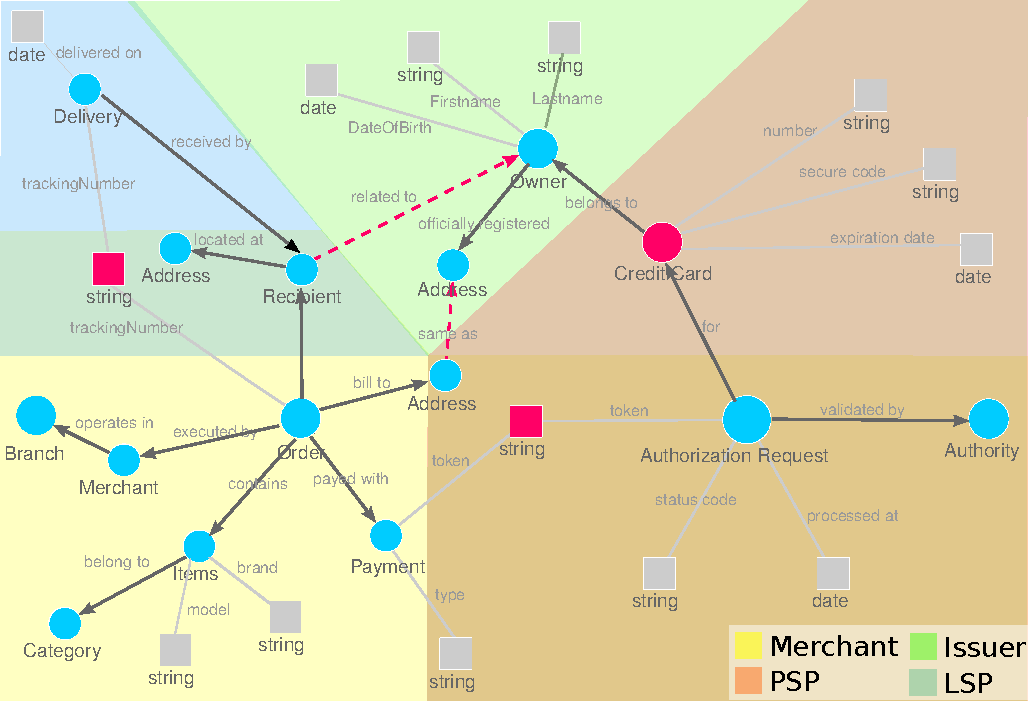
\includegraphics[width=0.9\columnwidth]{images/ontology_scenario_1.pdf}
  \caption{Data relations between stakeholders (green: Issuer, red: \gls{PSP}, yellow: Merchant, blue: \gls{LSP})}
\label{fig:images_data_model}
\end{figure}

As one can see there are connection points between these stakeholders. Those can be used as a reference for doing the merging of the information. There are actually three major connection points: \@

\begin{enumerate}
  \item \textbf{payment token}: shared between merchant and \gls{PSP}
  \item \textbf{tracking number}: shared between merchant and \gls{LSP}
  \item \textbf{credit card}: shared between issuer and \gls{PSP}
\end{enumerate}

In addition to these connection points one can also see the validation points in the Figure~\ref{fig:images_data_model}. These are critical points that have an influence on the decision whether an E-commerce transaction is suspecious or not. The criterias are: \@

\begin{enumerate}
  \item \textbf{billing address}: the billing address of the order has to match the registered address of the owner of the credit card used
  \item \textbf{recipient}: the recipient of the delivery has to be related to the owner of the credit card
\end{enumerate}

Whereas the first criteria can be examined during the authorization process of the credit card payment based on the information transmitted between merchant and \gls{PSP}, the second one is more difficult to validate (or can not be verified at all). The only check the \gls{LSP} is able to do before handing over the packaged items to the recipient, is to verify that she is the one mentioned in the order. If she is somehow related to the owner of the credit card or just a fraudster misusing the credit card data can not be confirmed at that point. \\

Also the merchant, the \gls{PSP} and the issuer are out of luck here. Whereas the merchant is able to validate whether the consumer has send items to that shipping address before, she can not restrict the consumer to choose only validated recipient addresses for shipping the order. Doing so will have a negative impact on the business of the online merchant. The \gls{PSP} and the issuer can not analyze this either, as both participants will not receive the information about the delivery address of the order in the credit card authorization request. \\

But just sharing the fact whether the shipping and billing address is different between the relevant stakeholders is not enough. Although this information is necessary, it is not sufficient to make a decision about suspecious transactions. Other necessary information are whether the consumer has send orders to this shipping address before, and the information about the content of the current order. Still, as mentioned in Section~\ref{sec:scope_thesis} looking at the single transaction of one merchant is not enough in the E-commerce fraud scenario that this thesis looks at. \\

Therefore the idea is to combine the transaction information from various merchants, \gls{LSP}s, \gls{PSP}s and issuers into one large, combined and shared information space to be able to analyze if there are any orders that look strange and are not being made by the owner of the credit card to a certain extend. One can already see that the proposed solution will have to deal with statistical evaluations and probabilities. \\

Starting with the credit card in question the issuer can query for the order details of transactions, that have been done recently with the credit card online. For that she might have to query the \gls{PSP} for the payment token first, before asking the merchant for order details to that payment token. At the end each online transaction can be mapped into a schema like the one shown in Figure~\ref{fig:images_data_model}, building up a large graph of entities and  the relationship between them, with the specific credit card in the center of it. An abbreviated sample graph of that can be seen in Figure~\ref{fig:images_credit_card_graph}. One can clearly recognize the different clusters of transactions by merchant. Still this first combination of the various order information into one data set is just the beginning of the analysis. Based on the information received the issuer can already filter out transactions, that have been shipped to different addresses than the credit card owner is registered for. Especially for those cases it might be worth to ask for additional information from the affected merchants to figure out if the consumer has used these shipping addresses before. As a result the existing graph can be enriched with additional transactional information from merchants at any time, if needed. In addition to the address information the issuer can also analyse the item information (incl.\ category, brand and model) of each order. \\

\begin{figure}[!ht]
  \centering
  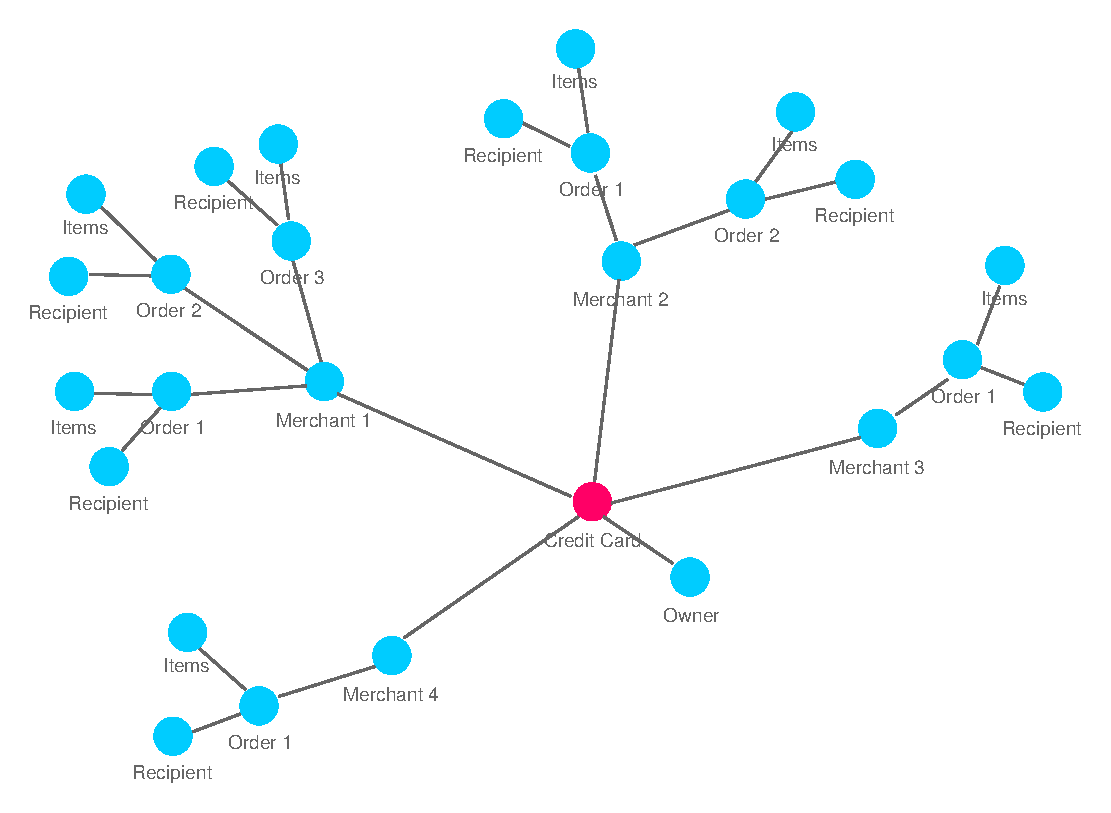
\includegraphics[width=0.9\columnwidth]{images/ontology_scenario_2.pdf}
  \caption{Clusters of E-commerce transactions by merchant}
\label{fig:images_credit_card_graph}
\end{figure}

But as shown in the Section~\ref{sec:scope_thesis} analysing the cluster of transactions from each merchant \textbf{\underline{alone}} will not be sufficient to come up with a solid decision about a suspecious transaction. This is due to the usage pattern of the fraudsters, that have been described in the scenario selected for this Master thesis --- using a credit card for ordering items from multiple merchants online. Therefore the various order details from the merchants have to be mapped against each other, so that the initial graph can be easily transformed into additional representations that uses different criterias to cluster the transactions --- such as recipient addresses, branches of the merchants, or product-related information. This reshaping of the graph can lead to new insights about the ``normal'' shopping behaviour of the credit card owner and make deviations from this behaviour visible. Visualizing the graph data as a clustered graph on screen supports the explorative nature of knowledge generation and perception, and can speed up the investigation of the E-commerce fraud incidents. An example visualization of a clustered graph is shown in Figure~\ref{fig:images_graph_viz}. \@

\begin{figure}[H]
  \centering
  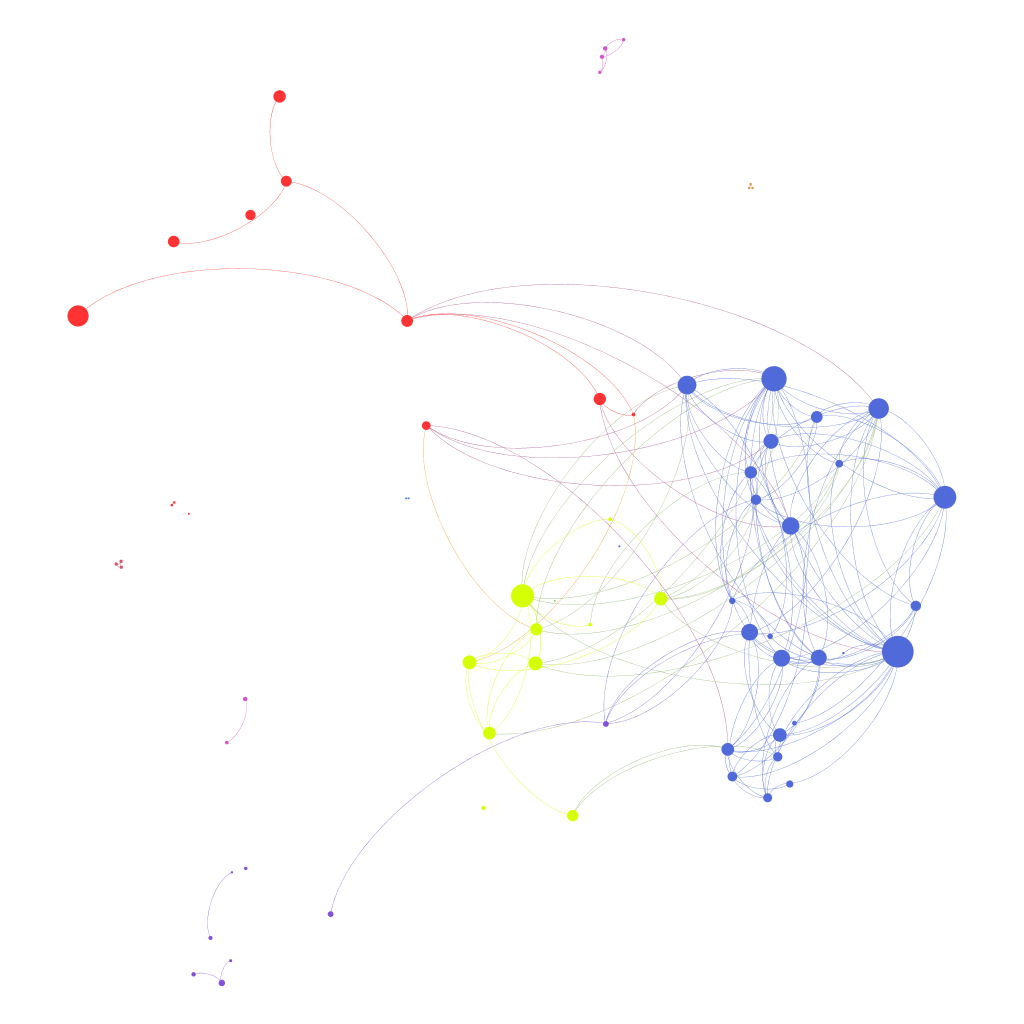
\includegraphics[width=0.9\columnwidth]{images/GraphViz.png}
  \caption{An example visualization of a clustered graph \citep{visjsshowcase}}
\label{fig:images_graph_viz}
\end{figure}

 In addition to these clustered graphs the system can also support the investigation of the incidents by changing the type of visualization based on the criteria chosen for the clustering of the order details; e.g.\ when clustering them based on location information such as the shipping addresses the system can present the information as a heat map on a chart as displayed in Figure~\ref{fig:images_map_heatmap}. \@

\begin{figure}[H]
  \centering
  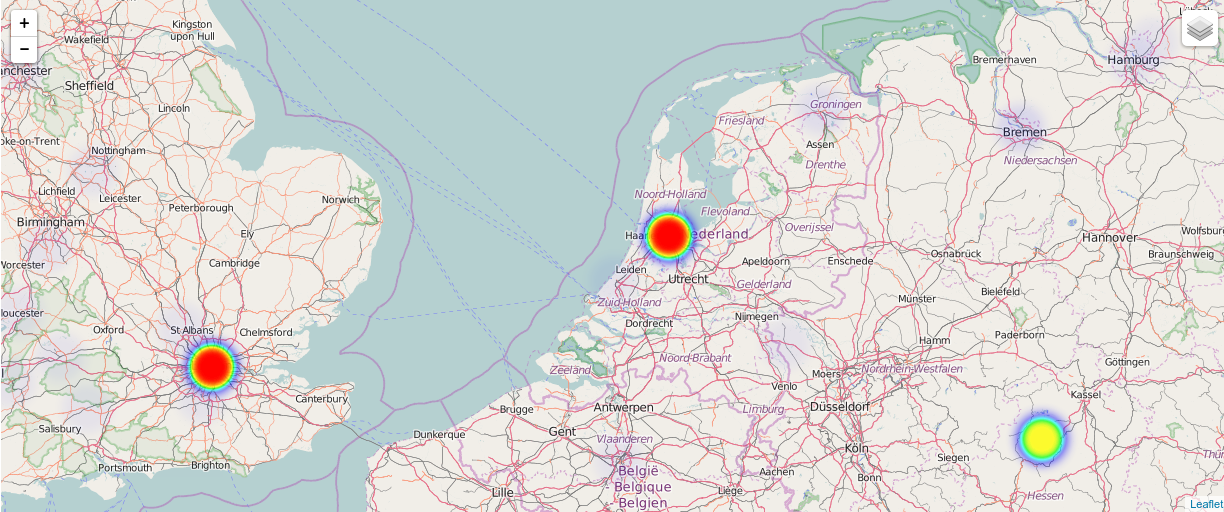
\includegraphics[width=0.9\columnwidth]{images/Heatmap.png}
  \caption{Heatmap displaying clusters of location-based information}
\label{fig:images_map_heatmap}
\end{figure}

To conclude the system have to support the collection and combination of E-commerce transaction information from various sources into a large clustered graph, that can be analysed from multiple view points to validate if there is any transaction that stands out from the ``normal'' shopping behaviour of the credit card owner. The starting point is a sequence of recent credit card activities, that the issuer can provide to the other participants. The initial graph will collect and cluster the information from each merchant based on this list. In case there are suspecious information in one of the clusters of the merchant, the issuer can further enrich this cluster with additional historical order details for this customer from that merchant. In the final step the system has to do the mapping of the order detail information between each merchant to allow further analysing and clustering of the transactions. 

% section system_overview (end)
